%%%%%%%%%%%%  Generated using docx2latex.com  %%%%%%%%%%%%%%

%%%%%%%%%%%%  v2.0.0-beta  %%%%%%%%%%%%%%

\documentclass[a4paper,12pt]{article}

% Other options in place of 'report' are 1)article 2)book 3)letter
% Other options in place of 'a4paper' are 1)a5paper 2)b5paper 3)letterpaper 4)legalpaper 5)executivepaper


 %%%%%%%%%%%%  Include Packages  %%%%%%%%%%%%%%


\usepackage{amsmath}
\usepackage{latexsym}
\usepackage{amsfonts}
\usepackage[normalem]{ulem}
\usepackage{array}
\usepackage{amssymb}
\usepackage{graphicx}
\usepackage{subfig}
\usepackage{wrapfig}
\usepackage{wasysym}
\usepackage{enumitem}
\usepackage{adjustbox}
\usepackage{ragged2e}
\usepackage{longtable}
\usepackage{changepage}
\usepackage{setspace}
\usepackage{hhline}
\usepackage{multicol}
\usepackage{float}
\usepackage{multirow}
\usepackage{makecell}
\usepackage{fancyhdr}
\usepackage[toc,page]{appendix}
\usepackage[a4paper,left=0.79in,right=0.79in,top=0.79in,bottom=0.79in,headheight=1in]{geometry}
\usepackage[utf8]{inputenc}
\usepackage[T1]{fontenc}
\usepackage{color,hyperref}
\definecolor{darkblue}{rgb}{0.0,0.0,1}


 %%%%%%%%%%%%  Define Colors For Hyperlinks  %%%%%%%%%%%%%%


\urlstyle{same}


 %%%%%%%%%%%%  Set Depths for Sections  %%%%%%%%%%%%%%

% 1) Section
% 1.1) SubSection
% 1.1.1) SubSubSection
% 1.1.1.1) Paragraph
% 1.1.1.1.1) Subparagraph


\setcounter{tocdepth}{5}
\setcounter{secnumdepth}{5}


 %%%%%%%%%%%%  Set Page Margins  %%%%%%%%%%%%%%


\everymath{\displaystyle}


 %%%%%%%%%%%%  Set Depths for Nested Lists created by \begin{enumerate}  %%%%%%%%%%%%%%


\setlistdepth{9}
\newlist{custom_Enumerate}{enumerate}{9}
	\setlist[custom_Enumerate,1]{label=\arabic*)}
	\setlist[custom_Enumerate,2]{label=\alph*)}
	\setlist[custom_Enumerate,3]{label=(\roman*)}
	\setlist[custom_Enumerate,4]{label=(\arabic*)}
	\setlist[custom_Enumerate,5]{label=(\Alph*)}
	\setlist[custom_Enumerate,6]{label=(\Roman*)}
	\setlist[custom_Enumerate,7]{label=\arabic*}
	\setlist[custom_Enumerate,8]{label=\alph*}
	\setlist[custom_Enumerate,9]{label=\roman*}

\renewlist{itemize}{itemize}{9}
	\setlist[itemize]{label=$\cdot$}
	\setlist[itemize,1]{label=\textbullet}
	\setlist[itemize,2]{label=$\circ$}
	\setlist[itemize,3]{label=$\ast$}
	\setlist[itemize,4]{label=$\dagger$}
	\setlist[itemize,5]{label=$\triangleright$}
	\setlist[itemize,6]{label=$\bigstar$}
	\setlist[itemize,7]{label=$\blacklozenge$}
	\setlist[itemize,8]{label=$\prime$}



\begin{document}
\sloppy
\begin{FlushLeft}
{\fontsize{12pt}{12pt}\selectfont \begin{Center}
{\fontsize{24pt}{24pt}\selectfont Introduction to Machine Learning Project 1}}
\end{Center}\par

\begin{FlushLeft}
{\fontsize{12pt}{12pt}\selectfont {\fontsize{14pt}{14pt}\selectfont 0416324 資工系 胡安鳳 An-Fong Hwu ,Dept of Computer Science }}
\end{FlushLeft}\par

\begin{FlushLeft}
{\fontsize{12pt}{12pt}\selectfont \begin{FlushLeft}
{\fontsize{20pt}{20pt}\selectfont 1.Programming Environment}}
\end{FlushLeft}\par



%%%%%%%%%%%%%%%%%%%% Figure/Image No: 1 starts here %%%%%%%%%%%%%%%%%%%%

\begin{figure}[H]
	\begin{FlushLeft}
		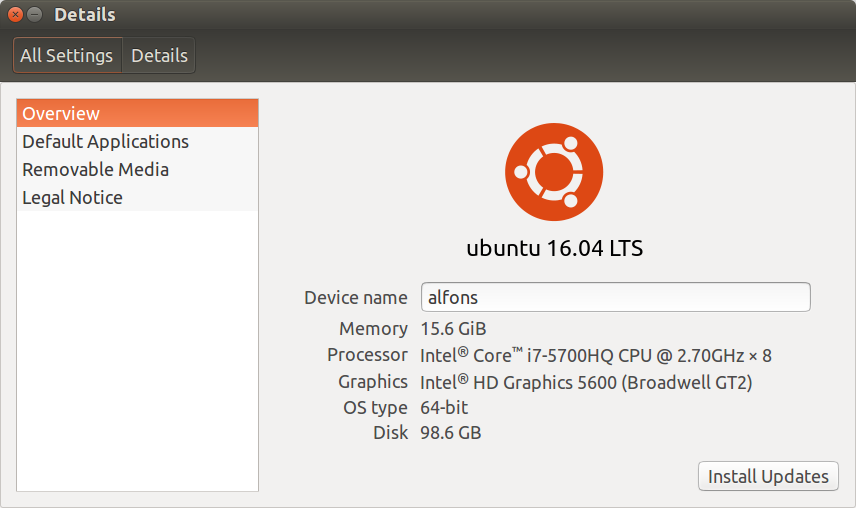
\includegraphics[width=3.89in,height=2.31in]{./media/image1.png}
	\end{FlushLeft}\end{figure}


%%%%%%%%%%%%%%%%%%%% Figure/Image No: 1 Ends here %%%%%%%%%%%%%%%%%%%%

\begin{FlushLeft}
{\fontsize{12pt}{12pt}\selectfont \begin{FlushLeft}
}
\end{FlushLeft}
\vspace{12pt}\begin{FlushLeft}
{\fontsize{12pt}{12pt}\selectfont \begin{FlushLeft}
{\fontsize{14pt}{14pt}\selectfont Programming language used: C++ with -std=c++11 standard and library with $\#$include <bits/stdc++.h>}}
\end{FlushLeft}\par

\begin{FlushLeft}
{\fontsize{12pt}{12pt}\selectfont \begin{FlushLeft}
{\fontsize{20pt}{20pt}\selectfont 2.What is Decision Tree and Random Forest?}}
\end{FlushLeft}\par

\begin{FlushLeft}
{\fontsize{12pt}{12pt}\selectfont \begin{FlushLeft}
}
\end{FlushLeft}
\vspace{12pt}\begin{FlushLeft}
{\fontsize{12pt}{12pt}\selectfont \begin{FlushLeft}
{\fontsize{14pt}{14pt}\selectfont A simple machine learning and training model for data prediction and analysis.}}
\end{FlushLeft}\par

\begin{FlushLeft}
{\fontsize{12pt}{12pt}\selectfont \begin{FlushLeft}
\href{https://en.wikipedia.org/wiki/Decision$ \_ $tree}{https://en.wikipedia.org/wiki/Decision$ \_ $tree}}
\end{FlushLeft}\par

\begin{FlushLeft}
{\fontsize{12pt}{12pt}\selectfont \begin{FlushLeft}
\href{https://en.wikipedia.org/wiki/Random$ \_ $forest}{https://en.wikipedia.org/wiki/Random$ \_ $forest}}
\end{FlushLeft}\par

\begin{FlushLeft}
{\fontsize{12pt}{12pt}\selectfont \begin{FlushLeft}
{\fontsize{20pt}{20pt}\selectfont 3.How decision tree is built?}}
\end{FlushLeft}\par

\begin{FlushLeft}
{\fontsize{12pt}{12pt}\selectfont \begin{FlushLeft}
}
\end{FlushLeft}
\vspace{12pt}\begin{FlushLeft}
{\fontsize{12pt}{12pt}\selectfont \begin{FlushLeft}
{\fontsize{14pt}{14pt}\selectfont 0.Store~the data into the set of vector  }}
\end{FlushLeft}\par

\begin{FlushLeft}
{\fontsize{12pt}{12pt}\selectfont \begin{FlushLeft}
{\fontsize{14pt}{14pt}\selectfont 1.Sort~according to the attribute (dose not matter which attribute will get the most information gain since all splitting and attribute will be calculated  ) }}
\end{FlushLeft}\par

\begin{FlushLeft}
{\fontsize{12pt}{12pt}\selectfont \begin{FlushLeft}
{\fontsize{14pt}{14pt}\selectfont 2.If different at index then we calculate at (or say split with (value[index]+value[index-1])/2) }}
\end{FlushLeft}\par

\begin{FlushLeft}
{\fontsize{12pt}{12pt}\selectfont \begin{FlushLeft}
{\fontsize{14pt}{14pt}\selectfont 3.Now the table has been split into 2 parts, then calculate $"$each splitting point$"$according to the ID3 algorithm}}
\end{FlushLeft}\par

\begin{FlushLeft}
{\fontsize{12pt}{12pt}\selectfont \begin{FlushLeft}
{\fontsize{14pt}{14pt}\selectfont By using the std::map, we will increase the convenience to make a statistics of dataset.}}
\end{FlushLeft}\par

\begin{FlushLeft}
{\fontsize{12pt}{12pt}\selectfont \begin{FlushLeft}
{\fontsize{14pt}{14pt}\selectfont After calculating the position of splitting with LEAST ENTROPY , which means the $"$chaos$"$ of data is the LEAST, then we split at such position to reduce the data inconsistency.}}
\end{FlushLeft}\par



%%%%%%%%%%%%%%%%%%%% Figure/Image No: 1 starts here %%%%%%%%%%%%%%%%%%%%

\begin{figure}[H]
	\begin{FlushLeft}
		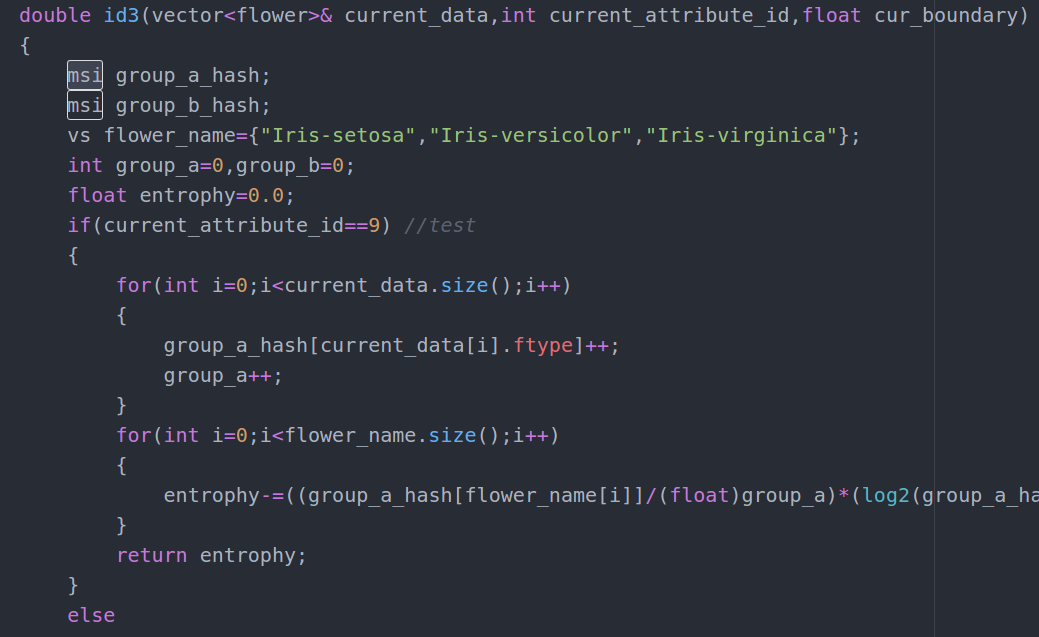
\includegraphics[width=6.69in,height=4.1in]{./media/image2.png}
	\end{FlushLeft}\end{figure}


%%%%%%%%%%%%%%%%%%%% Figure/Image No: 1 Ends here %%%%%%%%%%%%%%%%%%%%

\begin{FlushLeft}
{\fontsize{12pt}{12pt}\selectfont \begin{FlushLeft}
{\fontsize{14pt}{14pt}\selectfont  ~ }}
\end{FlushLeft}\par

\begin{FlushLeft}
{\fontsize{12pt}{12pt}\selectfont \begin{FlushLeft}
{\fontsize{14pt}{14pt}\selectfont 4.We~now have left$ \_ $child and right$ \_ $child. We split ,and  new* left$ \_ $child right child, connect them parent->newchild= something }}
\end{FlushLeft}\par

\begin{FlushLeft}
{\fontsize{12pt}{12pt}\selectfont \begin{FlushLeft}
{\fontsize{14pt}{14pt}\selectfont 6.take the needed data into leftchild which for example <180cm , then take all the person whose height <180cm into left child and vice versa for splitting the data set according to the current criterion.}}
\end{FlushLeft}\par

\begin{FlushLeft}
{\fontsize{12pt}{12pt}\selectfont \begin{FlushLeft}
}
\end{FlushLeft}
\vspace{12pt}\begin{FlushLeft}
{\fontsize{12pt}{12pt}\selectfont \begin{FlushLeft}
{\fontsize{14pt}{14pt}\selectfont Here is the code for putting the data in left child and right child}}
\end{FlushLeft}\par



%%%%%%%%%%%%%%%%%%%% Figure/Image No: 1 starts here %%%%%%%%%%%%%%%%%%%%

\begin{figure}[H]
	\begin{FlushLeft}
		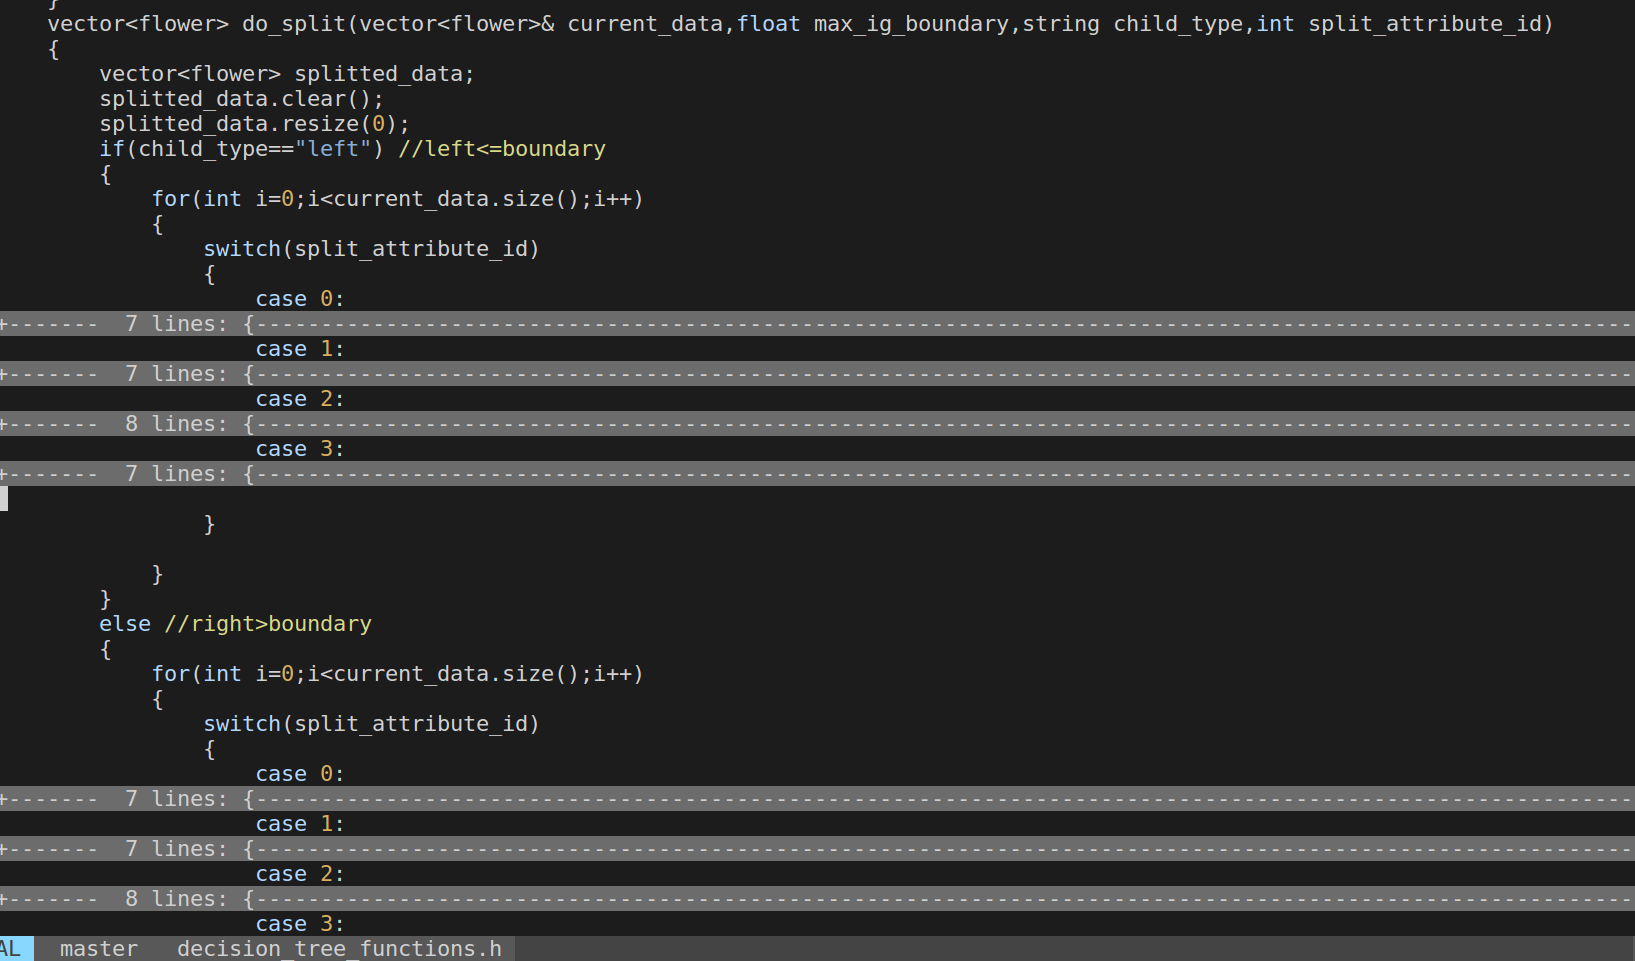
\includegraphics[width=6.69in,height=3.93in]{./media/image3.png}
	\end{FlushLeft}\end{figure}


%%%%%%%%%%%%%%%%%%%% Figure/Image No: 1 Ends here %%%%%%%%%%%%%%%%%%%%

\begin{FlushLeft}
{\fontsize{12pt}{12pt}\selectfont \begin{FlushLeft}
}
\end{FlushLeft}
\vspace{12pt}\begin{FlushLeft}
{\fontsize{12pt}{12pt}\selectfont \begin{FlushLeft}
{\fontsize{14pt}{14pt}\selectfont 5.If the node's data is homogeneous, stop (the node cannot be split even more). }}
\end{FlushLeft}\par

\begin{FlushLeft}
{\fontsize{12pt}{12pt}\selectfont \begin{FlushLeft}
{\fontsize{14pt}{14pt}\selectfont 6.the recursive algorithm is somehow like build$ \_ $decision$ \_ $tree(node* left$ \_ $child) build$ \_ $decision$ \_ $tree(node* right$ \_ $child) where the child is not null }}
\end{FlushLeft}\par



%%%%%%%%%%%%%%%%%%%% Figure/Image No: 1 starts here %%%%%%%%%%%%%%%%%%%%

\begin{figure}[H]
	\begin{FlushLeft}
		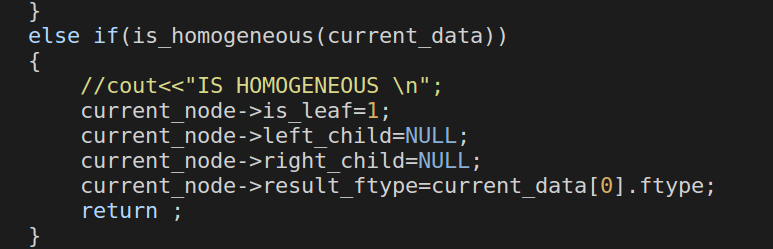
\includegraphics[width=4.77in,height=1.54in]{./media/image4.png}
	\end{FlushLeft}\end{figure}


%%%%%%%%%%%%%%%%%%%% Figure/Image No: 1 Ends here %%%%%%%%%%%%%%%%%%%%

\begin{FlushLeft}
{\fontsize{12pt}{12pt}\selectfont \begin{FlushLeft}
}
\end{FlushLeft}
\vspace{12pt}\begin{FlushLeft}
{\fontsize{12pt}{12pt}\selectfont \begin{FlushLeft}
}
\end{FlushLeft}
\vspace{12pt}\begin{FlushLeft}
{\fontsize{12pt}{12pt}\selectfont \begin{FlushLeft}
}
\end{FlushLeft}
\vspace{12pt}\begin{FlushLeft}
{\fontsize{12pt}{12pt}\selectfont \begin{FlushLeft}
}
\end{FlushLeft}
\vspace{12pt}\begin{FlushLeft}
{\fontsize{12pt}{12pt}\selectfont \begin{FlushLeft}
}
\end{FlushLeft}
\vspace{12pt}\begin{FlushLeft}
{\fontsize{12pt}{12pt}\selectfont \begin{FlushLeft}
}
\end{FlushLeft}
\vspace{12pt}\begin{FlushLeft}
{\fontsize{12pt}{12pt}\selectfont \begin{FlushLeft}
}
\end{FlushLeft}
\vspace{12pt}\begin{FlushLeft}
{\fontsize{12pt}{12pt}\selectfont \begin{FlushLeft}
{\fontsize{14pt}{14pt}\selectfont Q:Which attribute to split first? }}
\end{FlushLeft}\par

\begin{FlushLeft}
{\fontsize{12pt}{12pt}\selectfont \begin{FlushLeft}
{\fontsize{14pt}{14pt}\selectfont A:Does not matter, what matters is the boundary we split, the boundary has to bring us the most information gain }}
\end{FlushLeft}\par

\begin{FlushLeft}
{\fontsize{12pt}{12pt}\selectfont \begin{FlushLeft}
{\fontsize{14pt}{14pt}\selectfont  }}
\end{FlushLeft}\par

\begin{FlushLeft}
{\fontsize{12pt}{12pt}\selectfont \begin{FlushLeft}
{\fontsize{20pt}{20pt}\selectfont 3.Extend to Random Forest}}
\end{FlushLeft}\par

\begin{FlushLeft}
{\fontsize{12pt}{12pt}\selectfont \begin{FlushLeft}
{\fontsize{14pt}{14pt}\selectfont 0.Build 5 decision tree where data picked from the data which require 120 training sets}}
\end{FlushLeft}\par

\begin{FlushLeft}
{\fontsize{12pt}{12pt}\selectfont \begin{FlushLeft}
{\fontsize{14pt}{14pt}\selectfont 1.Each tree contains 96 datasets, reason is that 120/24=5 and 120-24=96, just like the K-Fold interval for one decision tree, but now we have the subinterval for 5 trees and 24 as a count number for interval.}}
\end{FlushLeft}\par

\begin{FlushLeft}
{\fontsize{12pt}{12pt}\selectfont \begin{FlushLeft}
{\fontsize{14pt}{14pt}\selectfont 2.Traverse the forest, the highest vote for the predicted class is the.}}
\end{FlushLeft}\par

\begin{FlushLeft}
{\fontsize{12pt}{12pt}\selectfont \begin{FlushLeft}
{\fontsize{14pt}{14pt}\selectfont 3.K Fold Cross validation still implementable.}}
\end{FlushLeft}\par

\begin{FlushLeft}
{\fontsize{12pt}{12pt}\selectfont \begin{FlushLeft}
{\fontsize{14pt}{14pt}\selectfont 4.Implement a set of root and using the same method to build the random forest}}
\end{FlushLeft}\par

\begin{FlushLeft}
{\fontsize{12pt}{12pt}\selectfont \begin{FlushLeft}
}
\end{FlushLeft}
\vspace{12pt}\begin{FlushLeft}
{\fontsize{12pt}{12pt}\selectfont \begin{FlushLeft}
}
\end{FlushLeft}
\vspace{12pt}\begin{FlushLeft}
{\fontsize{12pt}{12pt}\selectfont \begin{FlushLeft}
}
\end{FlushLeft}
\vspace{12pt}\begin{FlushLeft}
{\fontsize{12pt}{12pt}\selectfont \begin{FlushLeft}
}
\end{FlushLeft}
\vspace{12pt}\begin{FlushLeft}
{\fontsize{12pt}{12pt}\selectfont \begin{FlushLeft}
}
\end{FlushLeft}
\vspace{12pt}\begin{FlushLeft}
{\fontsize{12pt}{12pt}\selectfont \begin{FlushLeft}
}
\end{FlushLeft}
\vspace{12pt}\begin{FlushLeft}
{\fontsize{12pt}{12pt}\selectfont \begin{FlushLeft}
}
\end{FlushLeft}
\vspace{12pt}\begin{FlushLeft}
{\fontsize{12pt}{12pt}\selectfont \begin{FlushLeft}
}
\end{FlushLeft}
\vspace{12pt}\begin{FlushLeft}
{\fontsize{12pt}{12pt}\selectfont \begin{FlushLeft}
}
\end{FlushLeft}
\vspace{12pt}\begin{FlushLeft}
{\fontsize{12pt}{12pt}\selectfont \begin{FlushLeft}
}
\end{FlushLeft}
\vspace{12pt}\begin{FlushLeft}
{\fontsize{12pt}{12pt}\selectfont \begin{FlushLeft}
}
\end{FlushLeft}
\vspace{12pt}

%%%%%%%%%%%%%%%%%%%% Figure/Image No: 1 starts here %%%%%%%%%%%%%%%%%%%%

\begin{figure}[H]
	\begin{FlushLeft}
		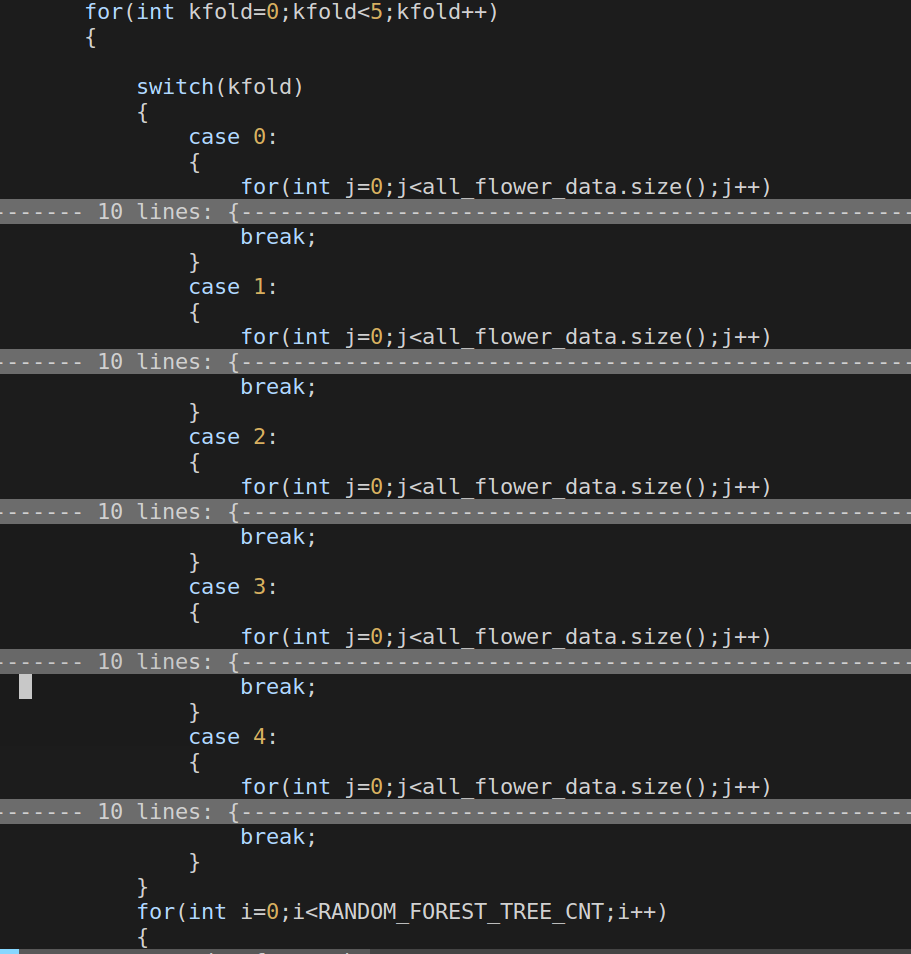
\includegraphics[width=3.02in,height=3.16in]{./media/image5.png}
	\end{FlushLeft}\end{figure}


%%%%%%%%%%%%%%%%%%%% Figure/Image No: 1 Ends here %%%%%%%%%%%%%%%%%%%%

\begin{FlushLeft}
{\fontsize{12pt}{12pt}\selectfont \begin{FlushLeft}
}
\end{FlushLeft}
\vspace{12pt}\begin{FlushLeft}
{\fontsize{12pt}{12pt}\selectfont \begin{FlushLeft}
}
\end{FlushLeft}
\vspace{12pt}\begin{FlushLeft}
{\fontsize{12pt}{12pt}\selectfont \begin{FlushLeft}
}
\end{FlushLeft}
\vspace{12pt}\begin{FlushLeft}
{\fontsize{12pt}{12pt}\selectfont \begin{FlushLeft}
}
\end{FlushLeft}
\vspace{12pt}\begin{FlushLeft}
{\fontsize{12pt}{12pt}\selectfont \begin{FlushLeft}
}
\end{FlushLeft}
\vspace{12pt}\begin{FlushLeft}
{\fontsize{12pt}{12pt}\selectfont \begin{FlushLeft}
}
\end{FlushLeft}
\vspace{12pt}

%%%%%%%%%%%%%%%%%%%% Figure/Image No: 1 starts here %%%%%%%%%%%%%%%%%%%%

\begin{figure}[H]
	\begin{FlushLeft}
		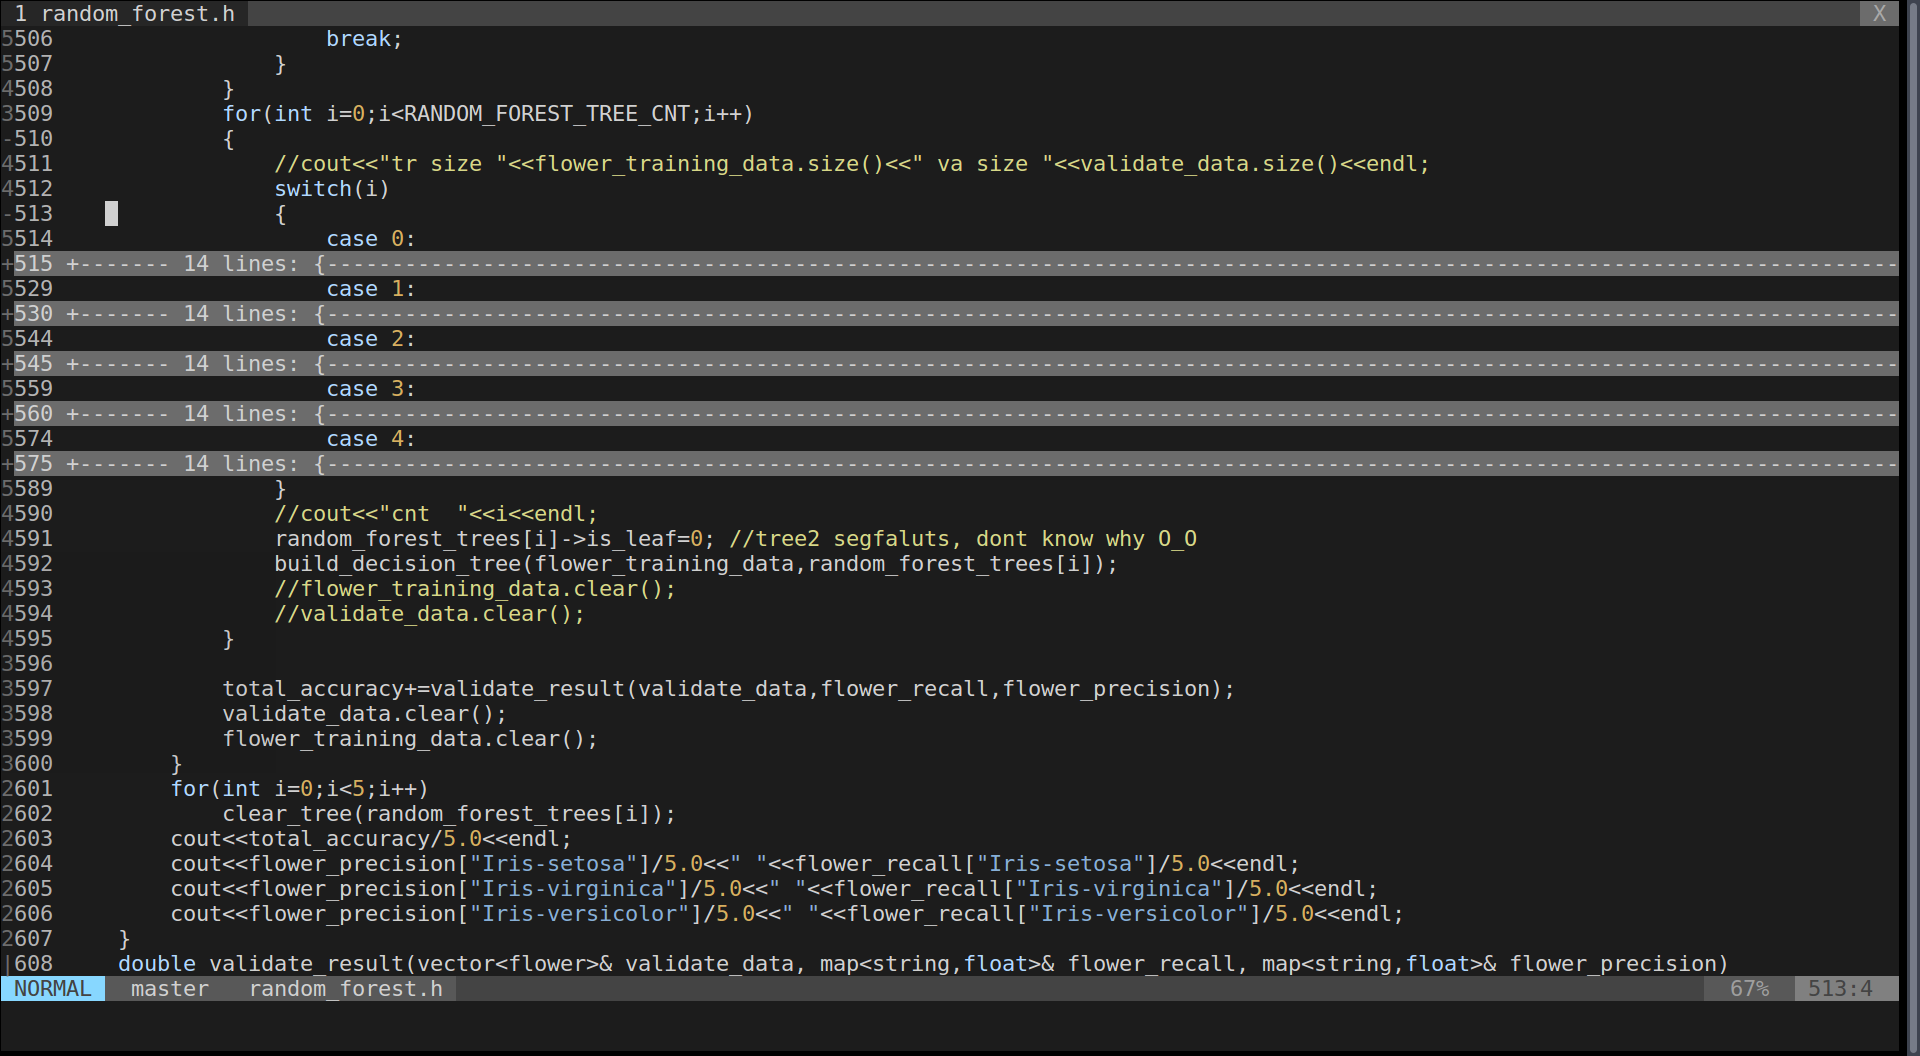
\includegraphics[width=5.74in,height=3.16in]{./media/image6.png}
	\end{FlushLeft}\end{figure}


%%%%%%%%%%%%%%%%%%%% Figure/Image No: 1 Ends here %%%%%%%%%%%%%%%%%%%%

\begin{FlushLeft}
{\fontsize{12pt}{12pt}\selectfont \begin{FlushLeft}
}
\end{FlushLeft}
\vspace{12pt}\begin{FlushLeft}
{\fontsize{12pt}{12pt}\selectfont \begin{FlushLeft}
}
\end{FlushLeft}
\vspace{12pt}\begin{FlushLeft}
{\fontsize{12pt}{12pt}\selectfont \begin{FlushLeft}
}
\end{FlushLeft}
\vspace{12pt}\begin{FlushLeft}
{\fontsize{12pt}{12pt}\selectfont \begin{FlushLeft}
}
\end{FlushLeft}
\vspace{12pt}\begin{FlushLeft}
{\fontsize{12pt}{12pt}\selectfont \begin{FlushLeft}
}
\end{FlushLeft}
\vspace{12pt}\begin{FlushLeft}
{\fontsize{12pt}{12pt}\selectfont \begin{FlushLeft}
}
\end{FlushLeft}
\vspace{12pt}\begin{FlushLeft}
{\fontsize{12pt}{12pt}\selectfont \begin{FlushLeft}
}
\end{FlushLeft}
\vspace{12pt}\begin{FlushLeft}
{\fontsize{12pt}{12pt}\selectfont \begin{FlushLeft}
}
\end{FlushLeft}
\vspace{12pt}\begin{FlushLeft}
{\fontsize{12pt}{12pt}\selectfont \begin{FlushLeft}
}
\end{FlushLeft}
\vspace{12pt}\begin{FlushLeft}
{\fontsize{12pt}{12pt}\selectfont \begin{FlushLeft}
}
\end{FlushLeft}
\vspace{12pt}\begin{FlushLeft}
{\fontsize{12pt}{12pt}\selectfont \begin{FlushLeft}
}
\end{FlushLeft}
\vspace{12pt}\begin{FlushLeft}
{\fontsize{12pt}{12pt}\selectfont \begin{FlushLeft}
}
\end{FlushLeft}
\vspace{12pt}\begin{FlushLeft}
{\fontsize{12pt}{12pt}\selectfont \begin{FlushLeft}
}
\end{FlushLeft}
\vspace{12pt}\begin{FlushLeft}
{\fontsize{12pt}{12pt}\selectfont \begin{FlushLeft}
{\fontsize{20pt}{20pt}\selectfont 4.Validate the Result}}
\end{FlushLeft}\par

\begin{FlushLeft}
{\fontsize{12pt}{12pt}\selectfont \begin{FlushLeft}
{\fontsize{14pt}{14pt}\selectfont There is a dramatically improved accuracy by using the Random Forest}}
\end{FlushLeft}\par



%%%%%%%%%%%%%%%%%%%% Figure/Image No: 1 starts here %%%%%%%%%%%%%%%%%%%%

\begin{figure}[H]
	\begin{FlushLeft}
		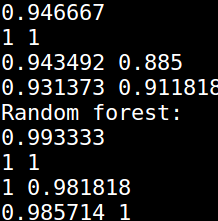
\includegraphics[width=1.82in,height=1.84in]{./media/image7.png}
	\end{FlushLeft}\end{figure}


%%%%%%%%%%%%%%%%%%%% Figure/Image No: 1 Ends here %%%%%%%%%%%%%%%%%%%%

\begin{FlushLeft}
{\fontsize{12pt}{12pt}\selectfont \begin{FlushLeft}
}
\end{FlushLeft}
\vspace{12pt}\begin{FlushLeft}
{\fontsize{12pt}{12pt}\selectfont \begin{FlushLeft}
}
\end{FlushLeft}
\vspace{12pt}\begin{FlushLeft}
{\fontsize{12pt}{12pt}\selectfont \begin{FlushLeft}
}
\end{FlushLeft}
\vspace{12pt}\begin{FlushLeft}
{\fontsize{12pt}{12pt}\selectfont \begin{FlushLeft}
}
\end{FlushLeft}
\vspace{12pt}\begin{FlushLeft}
{\fontsize{12pt}{12pt}\selectfont \begin{FlushLeft}
}
\end{FlushLeft}
\vspace{12pt}\begin{FlushLeft}
{\fontsize{12pt}{12pt}\selectfont \begin{FlushLeft}
{\fontsize{20pt}{20pt}\selectfont 5.Shell script}}
\end{FlushLeft}\par

\begin{FlushLeft}
{\fontsize{12pt}{12pt}\selectfont \begin{FlushLeft}
}
\end{FlushLeft}
\vspace{12pt}

%%%%%%%%%%%%%%%%%%%% Figure/Image No: 1 starts here %%%%%%%%%%%%%%%%%%%%

\begin{figure}[H]
	\begin{FlushLeft}
		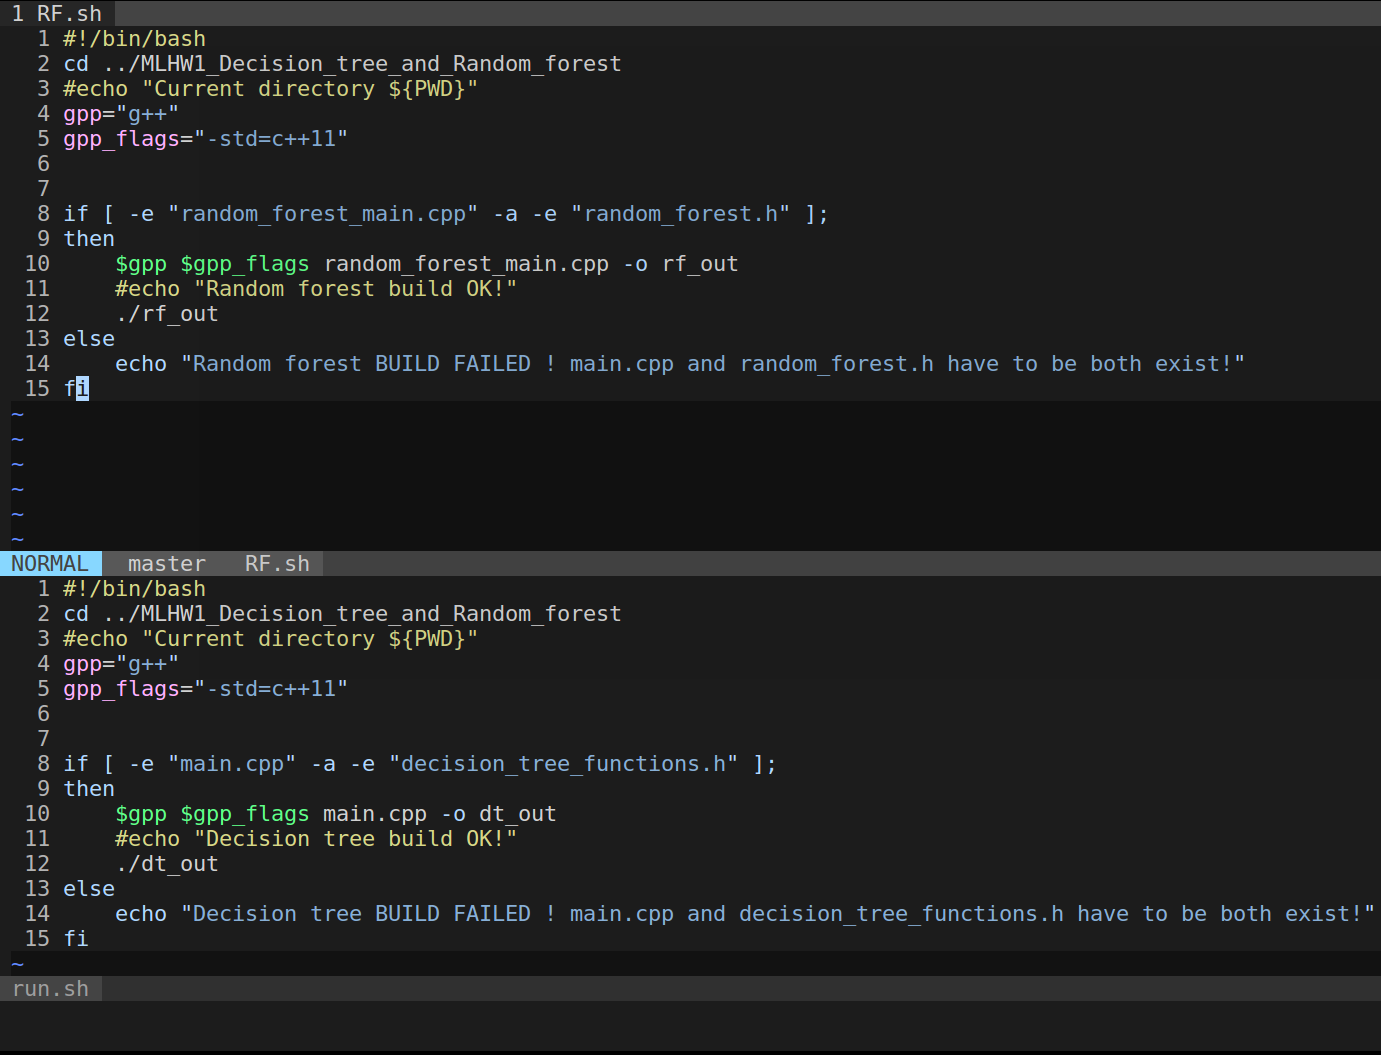
\includegraphics[width=6.69in,height=5.11in]{./media/image8.png}
	\end{FlushLeft}\end{figure}


%%%%%%%%%%%%%%%%%%%% Figure/Image No: 1 Ends here %%%%%%%%%%%%%%%%%%%%

\begin{FlushLeft}
{\fontsize{12pt}{12pt}\selectfont \begin{FlushLeft}
}
\end{FlushLeft}
\vspace{12pt}\begin{FlushLeft}
{\fontsize{12pt}{12pt}\selectfont \begin{FlushLeft}
{\fontsize{14pt}{14pt}\selectfont cd the relative path first ,setting the compiling flag, checking the availability of file then execute.}}
\end{FlushLeft}\par

\end{document}